% =====================================================================
%  1bat-ud6-9.tex  —  SESSIÓ 9: Consolidació de diagrames d'arbre
%  (sense preàmbul: s'inclou des de main.tex)
% =====================================================================
\horatitol{Sessió 9 — Consolidació de diagrames d'arbre}%
{Assentem la construcció i el càlcul amb arbres caçant els errors típics: branques que no sumen 1, multiplicar quan toca sumar, confondre l'ordre de la condicionada.}

\subsection{Idea clau}

Reforcem un dels procediments clau de la prova i un dels que més costa quan l'enunciat
té text: els \textbf{diagrames d'arbre}. No hi ha matèria nova; avui es tracta de
construir-los i recórrer-los \textbf{sense errors}, a partir d'enunciats de l'àmbit
social.

\begin{idea}
\textbf{Els tres errors que cacem avui}
\begin{enumerate}[leftmargin=1.6em, itemsep=2pt]
  \item \textbf{Branques que no sumen $1$:} d'un mateix node, les probabilitats han de
        sumar exactament $1$.
  \item \textbf{Multiplicar quan s'havia de sumar:} es \emph{multiplica} al llarg d'una
        ruta; se \emph{sumen} les rutes que porten al mateix resultat.
  \item \textbf{Confondre l'ordre de la condicionada:} la branca de la segona etapa
        depèn del que ha passat a la primera (no és la mateixa per a totes les rutes).
\end{enumerate}
\textbf{Rutina de comprovació:} a cada node, verifica que les branques sumen $1$; al
final, que totes les rutes completes sumen $1$.
\end{idea}

\subsection{Exemples}

\begin{exemple}[caça l'error: branques que no sumen 1]
Un arbre té, en un node, dues branques amb $0,6$ i $0,5$. \textbf{És incorrecte:}
$0,6+0,5=1,1>1$. Les branques d'un mateix node han de sumar $1$, de manera que si una
és $0,6$, l'altra ha de ser $0,4$ (no $0,5$). \textbf{Correcció:} $0,6$ i $0,4$.
\end{exemple}

\begin{exemple}[caça l'error: multiplicar en comptes de sumar]
Per calcular la probabilitat d'un resultat al qual porten \textbf{dues} rutes ($0,28$ i
$0,30$), algú fa $0,28\per 0,30=0,084$. \textbf{És incorrecte:} quan diferents rutes
porten al mateix resultat, se \textbf{sumen}:
\[
0,28+0,30=0,58.
\]
Es multiplica \emph{dins} d'una ruta (per encadenar etapes), no \emph{entre} rutes.
\textbf{Correcció:} $0,58$, no $0,084$.
\end{exemple}

\subsection{Exercicis resolts}

\begin{exresolt}[construir l'arbre d'una campanya]
Una campanya de prevenció: el $60\%$ dels joves hi assisteix; d'aquests, el $75\%$
\emph{no} recau. Dels que \textbf{no} hi assisteixen ($40\%$), només el $40\%$ no recau.
Construeix l'arbre i calcula la probabilitat que un jove \textbf{no recaigui}.
\solucio
\begin{center}
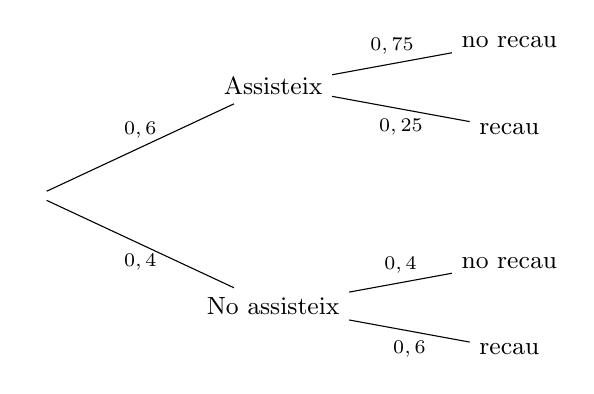
\begin{tikzpicture}[level distance=30mm, sibling distance=9mm,
   every node/.style={font=\small}, grow=right,
   level 1/.style={sibling distance=28mm},
   level 2/.style={sibling distance=11mm}]
\node {} 
  child {node {No assisteix}
    child {node {recau}      edge from parent node[below,font=\scriptsize]{$0,6$}}
    child {node {no recau}   edge from parent node[above,font=\scriptsize]{$0,4$}}
    edge from parent node[below,font=\scriptsize]{$0,4$}}
  child {node {Assisteix}
    child {node {recau}      edge from parent node[below,font=\scriptsize]{$0,25$}}
    child {node {no recau}   edge from parent node[above,font=\scriptsize]{$0,75$}}
    edge from parent node[above,font=\scriptsize]{$0,6$}};
\end{tikzpicture}
\end{center}
Sumem les dues rutes que porten a «no recau»:
\[
P(\text{no recau})=0,6\per 0,75+0,4\per 0,4=0,45+0,16=0,61.
\]
\resposta{$P(\text{no recau})=0,61$ ($61\%$).}
\end{exresolt}

\begin{exresolt}[una ruta concreta i la comprovació]
Amb l'arbre anterior, calcula la probabilitat de la ruta «assisteix i recau» i comprova
que totes les rutes sumen $1$.
\solucio
Ruta «assisteix i recau»: $0,6\per 0,25=0,15$.

Totes les rutes: $0,6\per 0,75=0,45$; $0,6\per 0,25=0,15$; $0,4\per 0,4=0,16$;
$0,4\per 0,6=0,24$. Suma: $0,45+0,15+0,16+0,24=1$: correcte.
\resposta{Ruta «assisteix i recau» $=0,15$; totes les rutes sumen $1$.}
\end{exresolt}

\subsection{Exercicis per fer}

\noindent\textit{Itinerari: els exercicis 1–4 són la base (arbres de dues etapes); el 5
i el 6 són ampliació (tres etapes i interpretació).}

\begin{exercicis}
\begin{exlist}
  \item \textbf{(Caça l'error)} Digues si és correcte i, si no, corregeix-lo:
    \begin{enumerate}[label=\alph*), leftmargin=1.6em, topsep=2pt]
      \item «Les dues branques d'un node valen $0,7$ i $0,4$.»
      \item «Un resultat al qual porten les rutes $0,2$ i $0,3$ té probabilitat
            $0,2\per 0,3=0,06$.»
    \end{enumerate}
  \item Un procés d'acollida: el $50\%$ completa la fase 1; d'aquests, el $80\%$
        continua. Dels que no la completen, el $30\%$ continua igualment. Dibuixa
        l'arbre i calcula la probabilitat de \textbf{continuar}.
  \item Amb l'arbre de l'exercici 2, calcula la probabilitat de la ruta «completa i
        continua» i comprova que totes les rutes sumen $1$.
  \item D'un node surten dues branques: una és $0,35$. Quant val l'altra? I si d'un node
        en surten tres i dues valen $0,4$ i $0,25$?
  \item \textbf{(Ampliació — tres etapes)} Un procés té tres etapes encadenades amb
        probabilitats $0,8$, després $0,5$, després $0,6$ al llarg d'una ruta concreta.
        Quina és la probabilitat d'aquesta ruta completa?
  \item \textbf{(Ampliació — interpretació)} En l'exemple de la campanya, quina ruta
        aporta més «no recaigudes»: la dels que assisteixen o la dels que no? Què
        suggereix això sobre la utilitat de la campanya?
\end{exlist}
\end{exercicis}

% ---------------------------------------------------------------------
\begin{idea}
\textbf{Full d'autoavaluació} — marca amb sinceritat com et trobes, de cara a la prova:
\begin{center}
\renewcommand{\arraystretch}{1.4}
\begin{tabular}{p{8.2cm} c c c}
\toprule
\textbf{Sé fer\dots} & \textbf{Sol} & \textbf{Amb ajuda} & \textbf{Encara no} \\
\midrule
Construir un arbre a partir d'un enunciat & \rule{0.7cm}{0pt} & & \\
Comprovar que les branques d'un node sumen $1$ & & & \\
Multiplicar al llarg d'una ruta & & & \\
Sumar les rutes que porten al mateix resultat & & & \\
Comprovar que totes les rutes sumen $1$ & & & \\
\bottomrule
\end{tabular}
\end{center}
\end{idea}

\noindent\textbf{Atenció a la diversitat.} Si encara et costa, comença per l'\emph{itinerari
mínim} (arbres de dues etapes amb enunciats curts i guia per col·locar les
probabilitats); si ja domines la tècnica, fes les \emph{ampliacions} (arbres de tres
etapes).

% ---------------------------------------------------------------------
\fullsolucions{Sessió 9}
\begin{solucions}
\begin{sollist}
  \item (a) \textbf{Incorrecte}: $0,7+0,4=1,1>1$; si una és $0,7$, l'altra ha de ser
        $0,3$. \quad (b) \textbf{Incorrecte}: rutes diferents al mateix resultat se
        \textbf{sumen}: $0,2+0,3=0,5$ (no $0,06$).
  \item Rutes cap a «continua»: $0,5\per 0,8=0,4$ i $0,5\per 0,3=0,15$.
        $P(\text{continua})=0,4+0,15=0,55$.
  \item Ruta «completa i continua»: $0,5\per 0,8=0,4$. Totes les rutes: $0,4$;
        $0,5\per 0,2=0,1$; $0,5\per 0,3=0,15$; $0,5\per 0,7=0,35$. Suma:
        $0,4+0,1+0,15+0,35=1$: correcte.
  \item Dues branques: l'altra val $1-0,35=0,65$. Tres branques amb $0,4$ i $0,25$: la
        tercera val $1-0,4-0,25=0,35$.
  \item Ruta completa: $0,8\per 0,5\per 0,6=0,24$.
  \item Ruta «assisteix i no recau»: $0,45$; ruta «no assisteix i no recau»: $0,16$.
        Aporta més la dels que \textbf{assisteixen} ($0,45$). Suggereix que la campanya
        és \textbf{útil}: assistir-hi puja molt la probabilitat de no recaure ($75\%$
        contra $40\%$).
\end{sollist}
\end{solucions}
